\documentclass[tikz,border=5pt]{standalone}
\usetikzlibrary{arrows.meta,calc,angles,quotes}
\tikzset{
    arrow/.style = {-{Latex[length=1.8mm,width=1mm]}, line width=0.6pt},
    fwd/.style  = {-{Latex[length=1.8mm,width=1mm]}, line width=0.6pt},
    bwd/.style  = {{Latex[length=1.8mm,width=1mm]}-, line width=0.6pt},
    both/.style = {{Latex[length=1.8mm,width=1mm]}-{Latex[length=1.8mm,width=1mm]}, line width=0.6pt}
}

\begin{document}
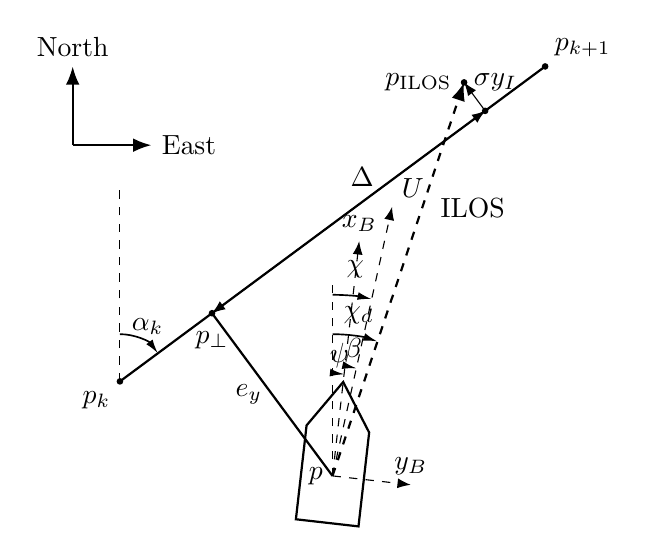
\begin{tikzpicture}[>=Latex]

    % ---------- helper NE axis ----------
    \coordinate (O) at (1.2,4.8);
    \draw[->, thick] (O) -- ++(0,1) node[above] {North};
    \draw[->, thick] (O) -- ++(1,0) node[right] {East};

    % =================================================
    % 1. Path, vehicle position, projection and look-ahead points
    % =================================================
    \coordinate (Pk)  at (1.8, 1.8);
    \coordinate (Pkp) at (7.2,5.8);
    \coordinate (P)   at (4.5,0.6);

    \draw[thick] (Pk) -- (Pkp);
    \fill (Pk)  circle (1.2pt);
    \fill (Pkp) circle (1.2pt);
    \node[below left]  at (Pk)  {$p_k$};
    \node[above right] at (Pkp) {$p_{k+1}$};

    % Orthogonal projection
    \coordinate (Pproj) at ($(Pk)!(P)!(Pkp)$);
    \fill (Pproj) circle (1.2pt);
    \node[below=3pt] at (Pproj) {$p_\perp$};

    % Nominal LOS point on the path
    \coordinate (Plos) at ($(Pproj)!0.82!(Pkp)$);
    \fill (Plos) circle (1.2pt);

    % Path angle (TikZ uses an East-based angle internally)
    \pgfmathanglebetweenpoints{\pgfpointanchor{Pk}{center}}{\pgfpointanchor{Pkp}{center}}
    \pgfmathsetmacro{\alphaE}{\pgfmathresult}

    % Virtual ILOS point: nominal LOS point plus a small integral offset.
    % Reverse both signs below if your cross-track convention is opposite.
    \def\Ishift{0.45}
    \coordinate (Pilos) at
      ($(Plos)+({-\Ishift*sin(\alphaE)},{\Ishift*cos(\alphaE)})$);
    \fill (Pilos) circle (1.2pt);
    \node[left=1pt] at (Pilos) {$p_{\mathrm{ILOS}}$};

    % Cross-track error and look-ahead distance
    \draw[thick] (P) -- (Pproj)
      node[pos=0.5, left] {$e_y$};
    \draw[<->] (Pproj) -- (Plos)
      node[pos=0.55, above=2pt] {$\Delta$};

    % Only one additional element distinguishes ILOS from LOS:
    % the integral compensation offset sigma*y_I.
    \draw[->] (Plos) -- (Pilos)
      node[above, right=0pt] {$\sigma y_I$};

    % Integral line-of-sight vector
    \draw[->,thick,dashed] (P) -- (Pilos)
      node[pos=0.68,right=3pt] {ILOS};

    % =================================================
    % 2. Local North reference lines
    % =================================================
    \coordinate (NorthRefP)  at ($(P)+(0,2.5)$);
    \coordinate (NorthRefPk) at ($(Pk)+(0,2.5)$);
    \draw[dashed] (P)  -- (NorthRefP);
    \draw[dashed] (Pk) -- (NorthRefPk);

    % =================================================
    % 3. Directions and vessel
    % =================================================
    \pgfmathanglebetweenpoints{\pgfpointanchor{P}{center}}{\pgfpointanchor{Pilos}{center}}
    \pgfmathsetmacro{\chiDE}{\pgfmathresult}

    \pgfmathsetmacro{\chiE}{\chiDE + 6}
    \pgfmathsetmacro{\psiE}{\chiE  + 6}

    \coordinate (ChiPoint) at ($(P)+({3.5*cos(\chiE)},{3.5*sin(\chiE)})$);
    \coordinate (PsiPoint) at ($(P)+({3.2*cos(\psiE)},{3.2*sin(\psiE)})$);

    \def\L{2.4}
    \def\B{0.8}
    \def\Lrect{1.2}

    \begin{scope}[shift={(P)}, rotate=\psiE]
        \coordinate (SternL) at (-\Lrect/2, -\B/2);
        \coordinate (SternR) at (-\Lrect/2,  \B/2);
        \coordinate (BowR)   at ( \Lrect/2,  \B/2);
        \coordinate (BowTip) at ( \L/2,      0);
        \coordinate (BowL)   at ( \Lrect/2, -\B/2);

        \draw[thick] (SternL) -- (SternR) -- (BowR) -- (BowTip) -- (BowL) -- cycle;
        \draw[->,dashed] (0,0) -- (3,0) node[above] {$x_B$};
        \draw[->,dashed] (0,0) -- (0,-1) node[above] {$y_B$};
    \end{scope}

    \node[left] at (P) {$p$};
    \draw[->,dashed] (P) -- (ChiPoint) node[above right] {$U$};

    % =================================================
    % 4. Angle annotations, measured clockwise from North
    % =================================================
    \draw pic[
      draw,bwd,angle radius=6mm,angle eccentricity=1.3,"$\alpha_k$"
    ] {angle = Pkp--Pk--NorthRefPk};

    \draw pic[
      draw,bwd,angle radius=13mm,angle eccentricity=1.18,"$\psi$"
    ] {angle = PsiPoint--P--NorthRefP};

    \draw pic[
      draw,bwd,angle radius=18mm,angle eccentricity=1.15,"$\chi_d$"
    ] {angle = Pilos--P--NorthRefP};

    \draw pic[
      draw,bwd,angle radius=23mm,angle eccentricity=1.15,"$\chi$"
    ] {angle = ChiPoint--P--NorthRefP};

    \draw pic[
      draw,bwd,angle radius=14mm,angle eccentricity=1.15,"$\beta$"
    ] {angle = ChiPoint--P--PsiPoint};

\end{tikzpicture}
\end{document}
